\documentclass{article}
\usepackage{graphicx, fancyhdr, amsmath}
\usepackage[margin=0.6in, top=1in]{geometry}
\usepackage{float}
\usepackage[absolute, overlay]{textpos}
\usepackage[colorlinks=true, linkcolor=blue]{hyperref}

\pagestyle{fancy}
\fancyhf{}
\renewcommand{\headrulewidth}{0pt}

\fancyhead[L]{
\begin{textblock*}{2cm}(0.3in,0.1in)  % {block width} (x-coordinate, y-coordinate)
    
\includegraphics[width=2cm]{NEW LOGO.png}  % Example image placeholder
\end{textblock*}
}
\fancyhead[R]{Math Success Program, UCLA}
\fancyfoot[R]{Created for the MSP by Asmi Kawatkar}

\fancypagestyle{plain}{
}


\title{Review Sheet: Improper Integrals}
\date{}
\author{}

\begin{document}
\maketitle
\vspace{-0.75in}
\section*{Content Review}
\subsection*{Overview}

Improper integrals are said to be 
\begin{itemize}
    \item convergent if the limit is finite and that limit is the value of the improper integral
    \item divergent if the limit does not exist
\end{itemize}

\noindent To simplify, if the limit exists, we say the improper integral \textbf{converges}. If either the limit fails to exist or is infinite, then the integral \textbf{diverges}.
\vspace{0.05in}
\newline\noindent A formal definition is:

Let $f(x)$  be continuous over an interval of the form $[a, +\infty)$. Then (provided this limit exists):
$$\int_a^{+\infty}{f(x)}dx = \lim_{t \rightarrow +\infty}{\int_a^t{f(x)}dx}$$

Let $f(x)$ be continuous over an interval of the form $(-\infty, b]$. Then (provided this limit exists):
$$\int_{-\infty}^{b}{f(x)}dx = \lim_{t \rightarrow -\infty}{\int_t^b{f(x)}dx}$$

Let $f(x)$ be continuous over $(-\infty, +\infty)$. Then
$$\int_{-\infty}^{+\infty}{f(x)}dx = \int_{-\infty}^0{f(x)}dx + \int_0^{+\infty}{f(x)}dx$$ provided that both integrals on the R.H.S converge. If either of these two integrals diverge, then their sum diverges.

\begin{figure}[H]
    \centering
    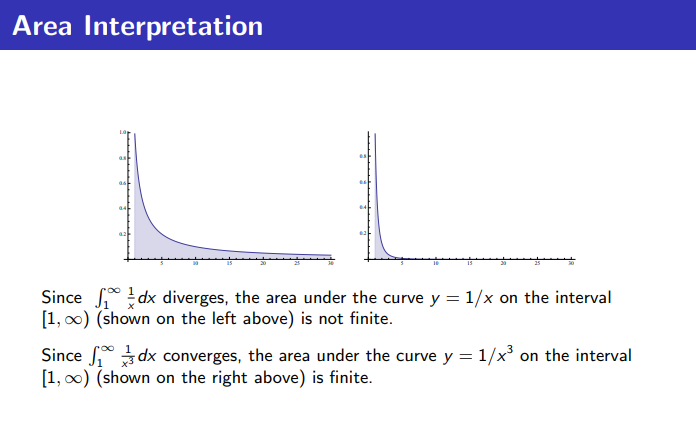
\includegraphics[width=0.7\linewidth]{Src1.png}
    \label{fig:Src1}
\end{figure}
\noindent\href{https://www3.nd.edu/~apilking/Math10560/Lectures/Lecture%2015.pdf}{Source for image}
\newline Skip to \hyperlink{WorkedProblems}{Worked Problems}



\subsection*{Resources}
\noindent\textit{Improper Integrals}
\begin{itemize}
    \item \href{https://tutorial.math.lamar.edu/classes/calcii/improperintegrals.aspx}{Notes: Paul's Online Notes}
    \item \href{https://www.khanacademy.org/math/ap-calculus-bc/bc-integration-new/bc-6-13/v/introduction-to-improper-integrals}{Introduction to Improper Integrals (Khan Academy)}
    \item \href{https://www.sfu.ca/math-coursenotes/Math%20158%20Course%20Notes/sec_ImproperIntegrals.html}{Notes + Practice Questions: Simon Fraser University}
    \item \href{https://youtu.be/ND9cEdfCFr0}{Video: Improper Integrals - Convergence and Divergence (Organic Chemistry Tutor - 14 min)}
    \item \href{https://tutorial.math.lamar.edu/problems/calcii/improperintegrals.aspx}{Practice Problems with Solutions: Paul's Online Notes}
\end{itemize}


\subsection*{Acknowlegement}
Questions in the Worked Problems section of this sheet have been taken from external sources that have been linked where appropriate. All solutions have been created independently.

\pagebreak
\section*{Worked Problems}
\hypertarget{WorkedProblems}{}

Determine if each of the following integrals converge or diverge. If the integral converges, determine its value
\newline \href{https://tutorial.math.lamar.edu/problems/calcii/improperintegrals.aspx}{Source} and \href{https://web.math.ucsb.edu/~vtkala/2014/Math3B/Math3B-ImproperIntegrals-Solutions.pdf}{Source} and \href{https://people.math.sc.edu/josephcf/Teaching/142/Files/Worksheets/Improper%20Integrals.pdf}{Source}

\begin{enumerate}
    \item $$\int_0^\infty{(1+2x)e^{-x}}dx$$
    \begin{figure}[H]
        \centering
        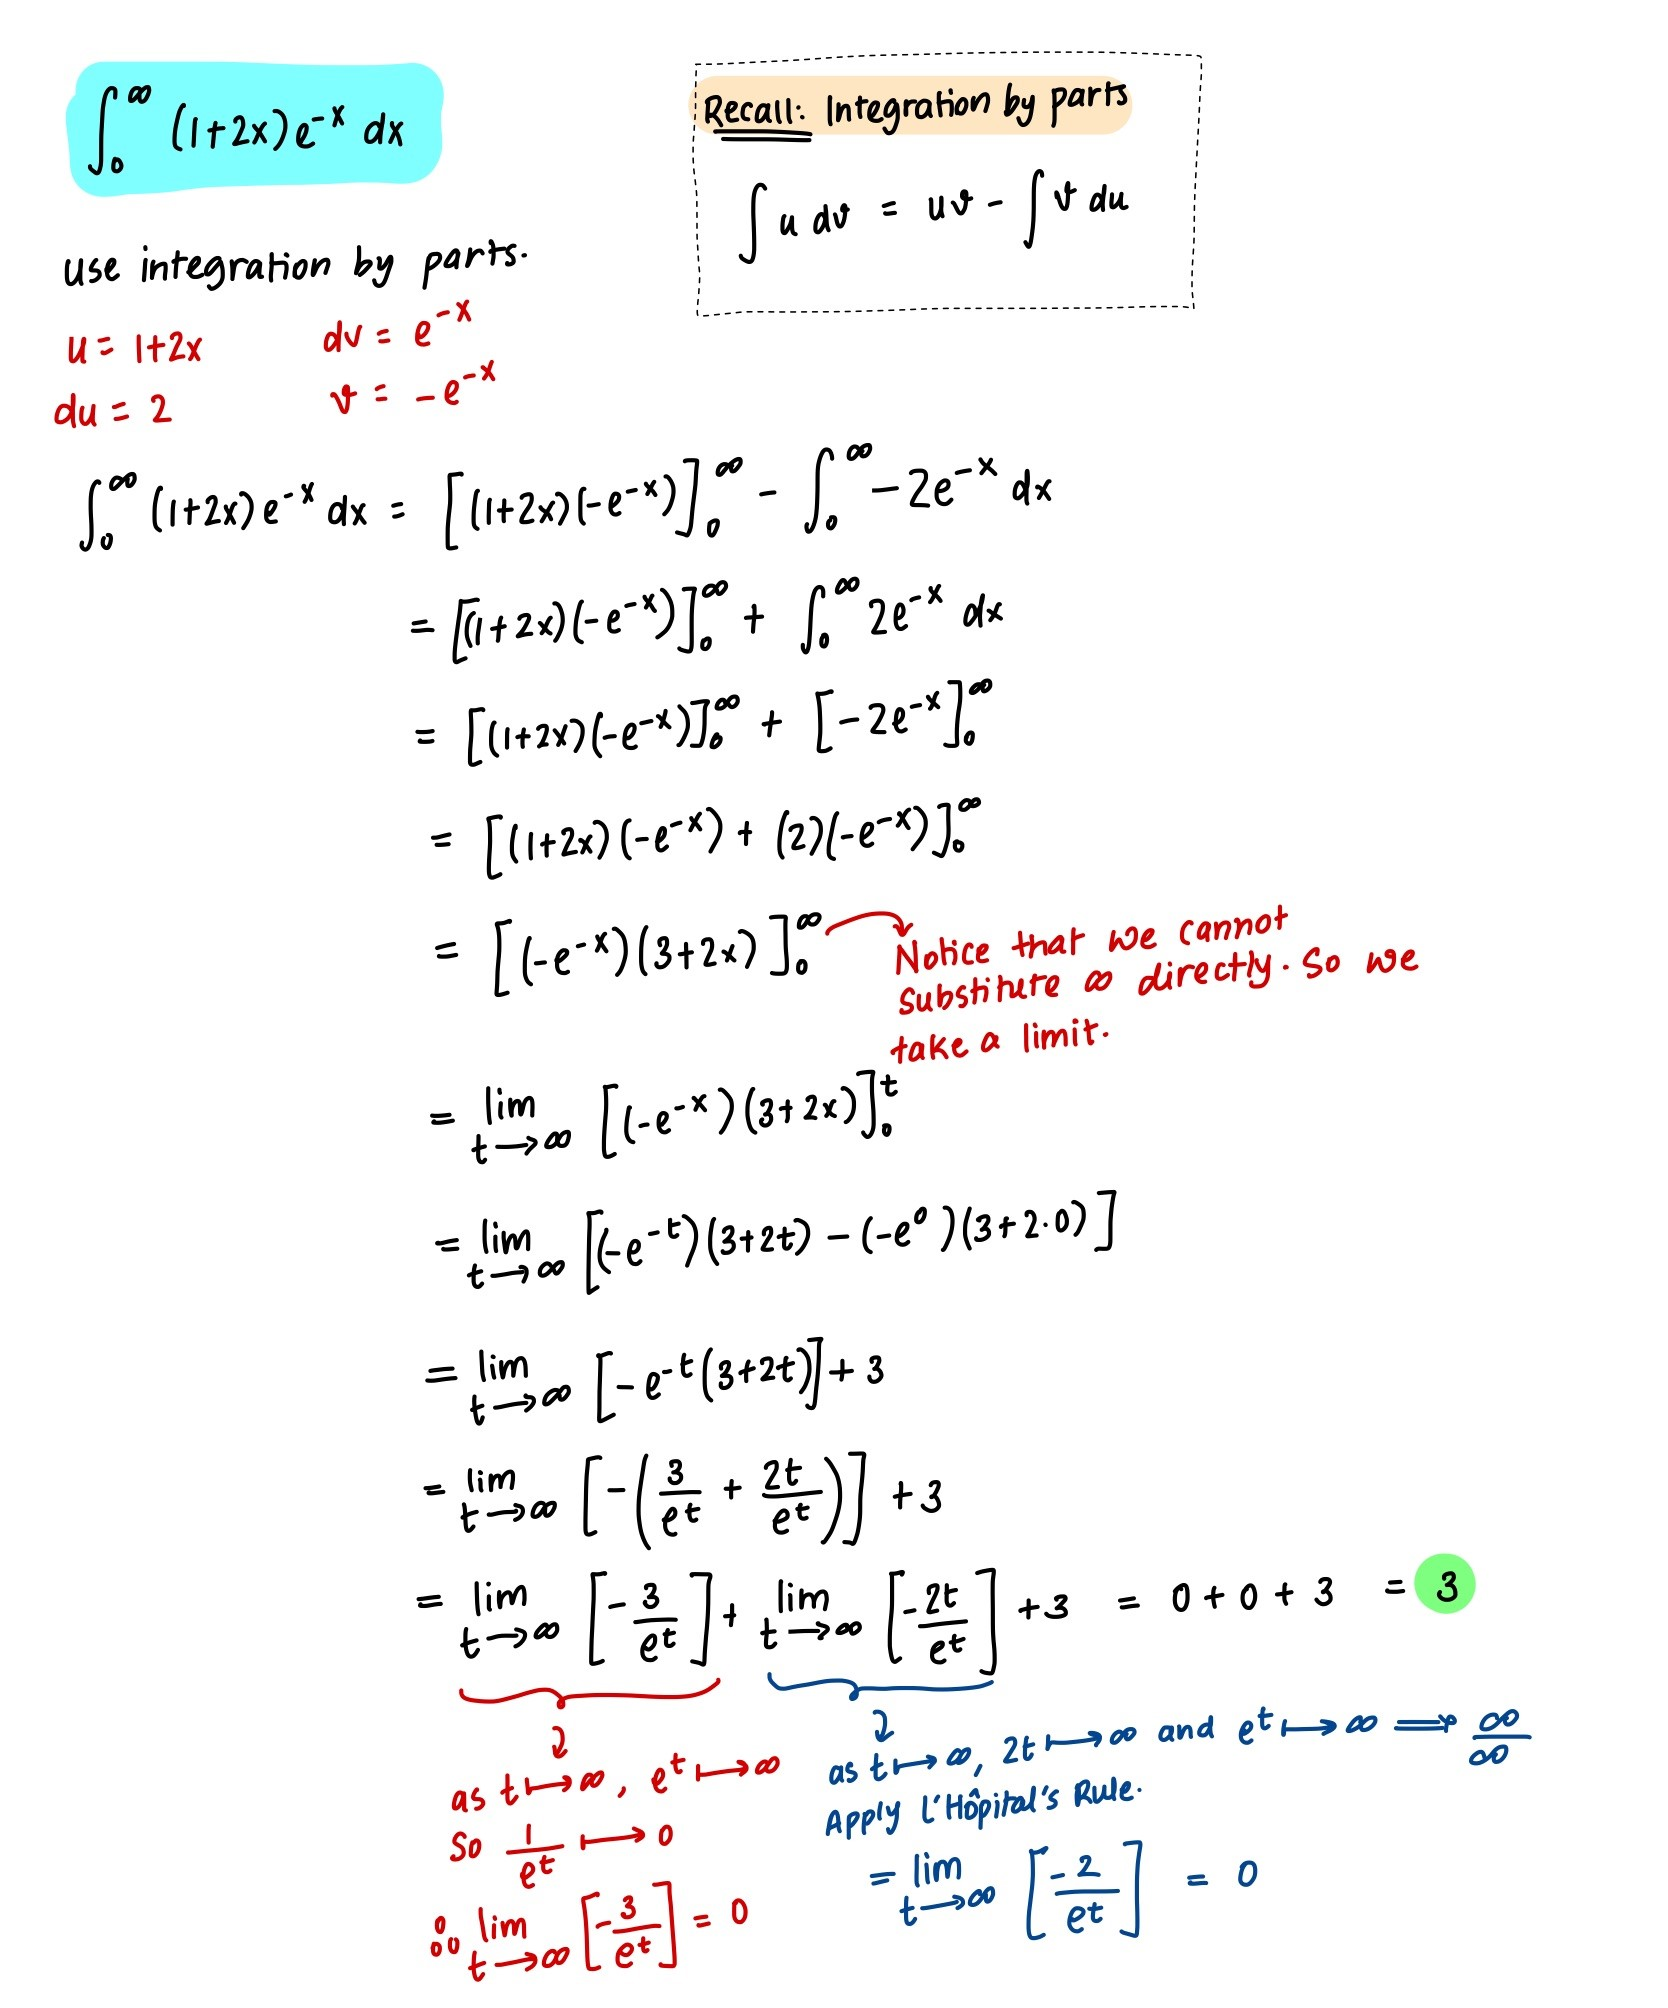
\includegraphics[width=0.9\linewidth]{Q1.jpg}
        \label{fig:Q1}
    \end{figure}
    \item $$\int_{-5}^1{\frac{1}{10+2z}}dz$$
    \begin{figure}[H]
        \centering
        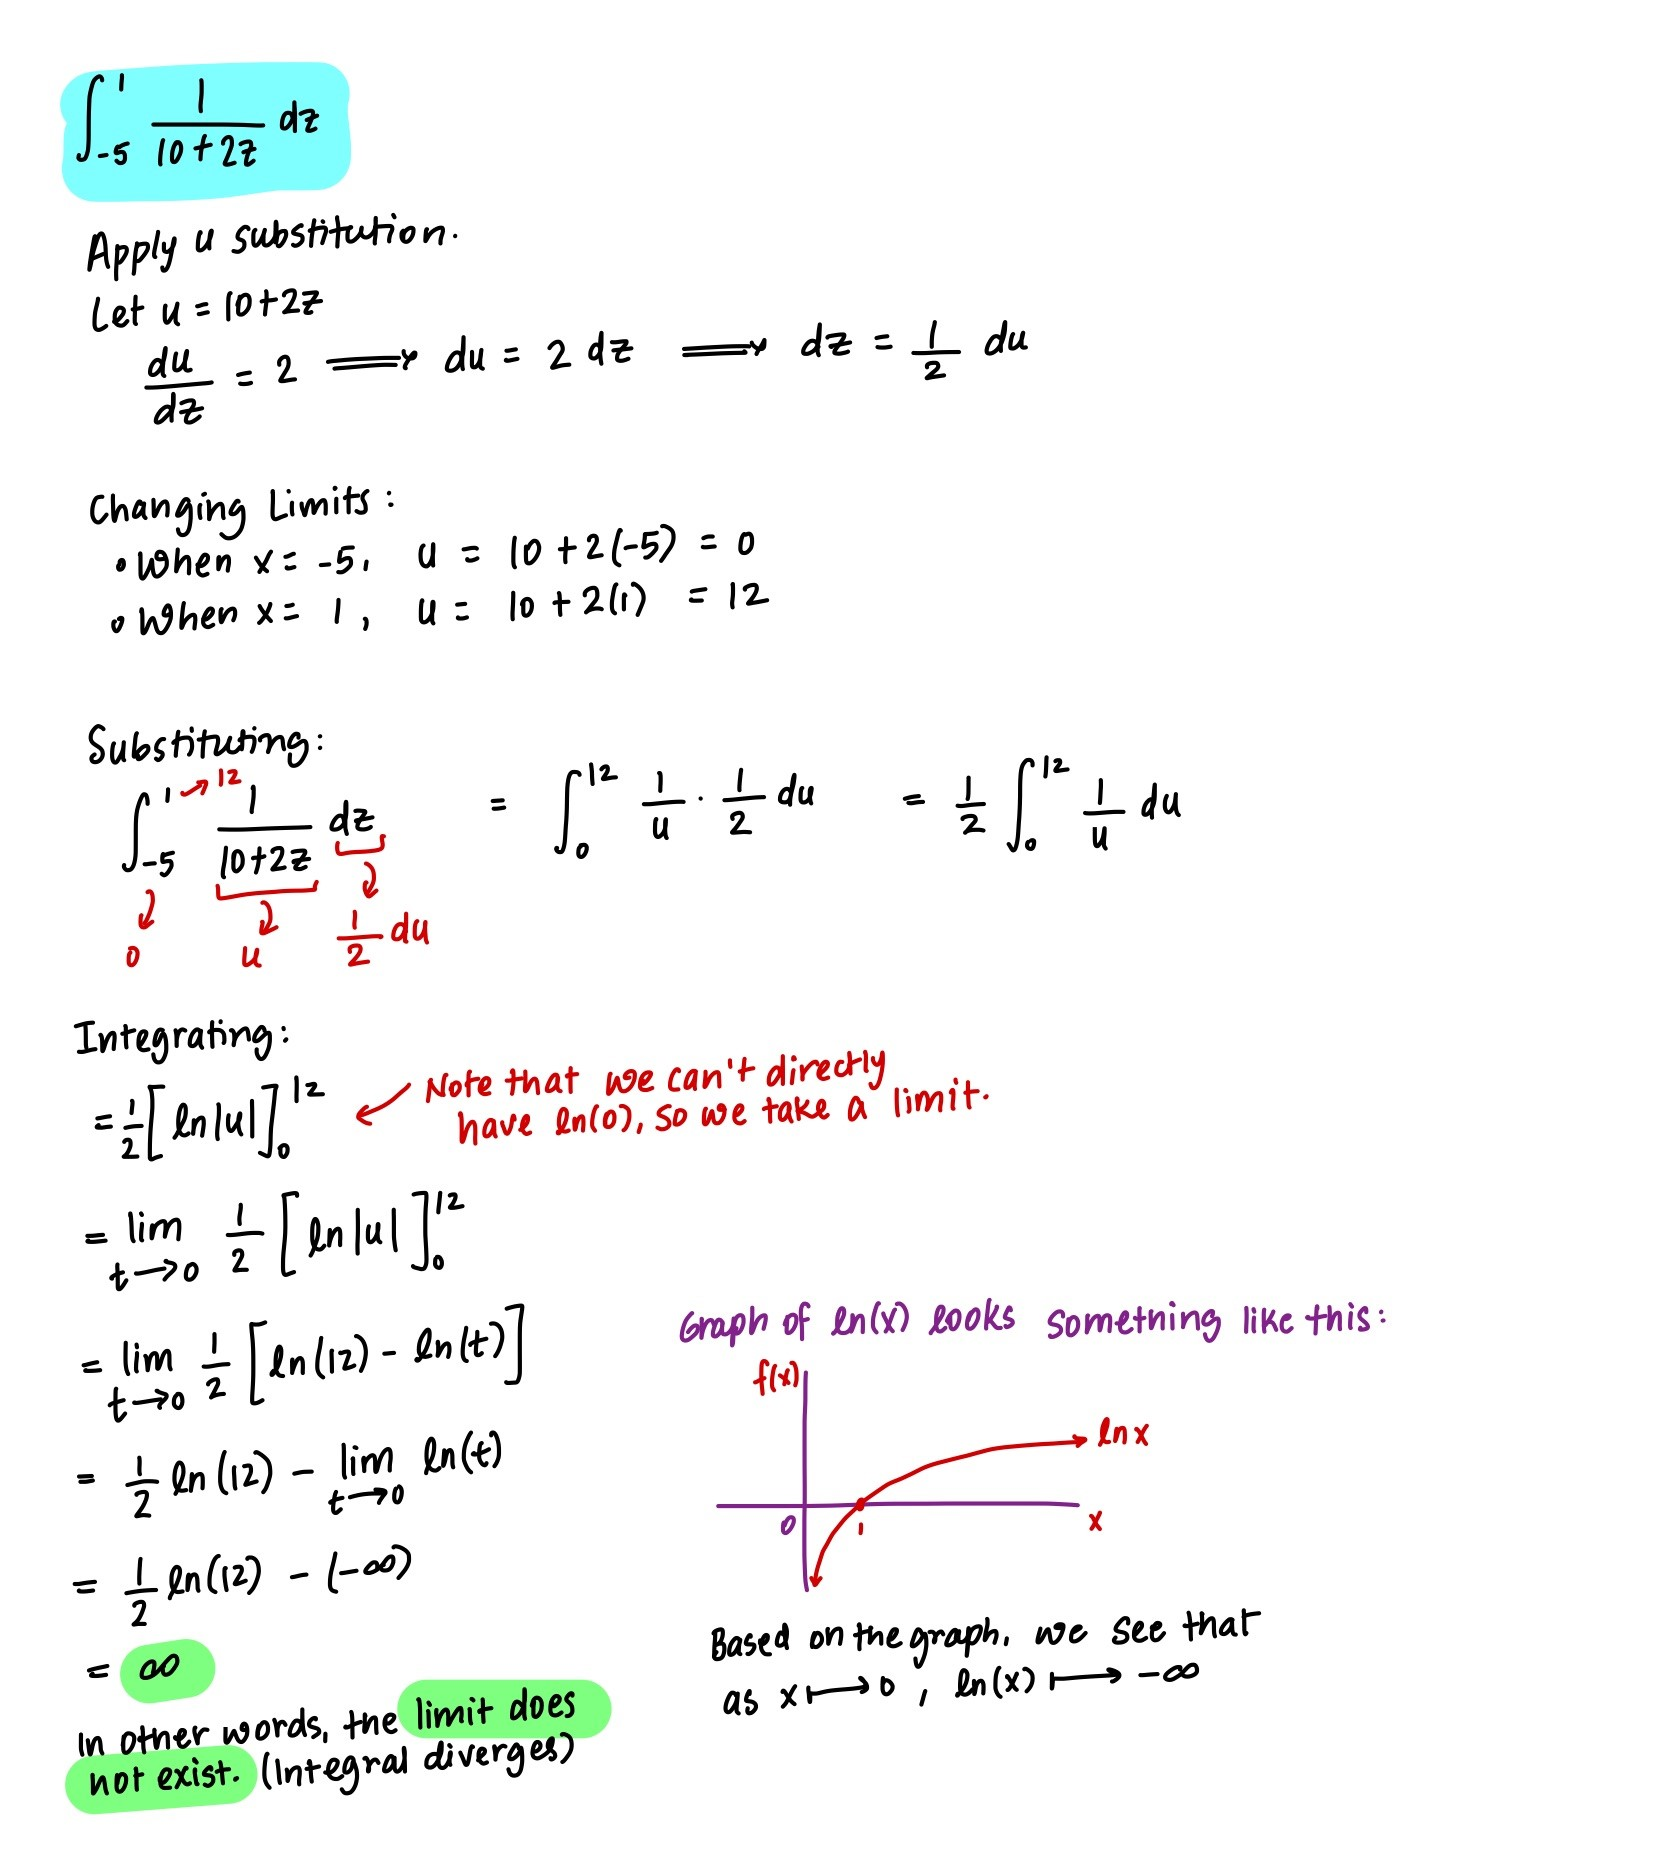
\includegraphics[width=\linewidth]{Q2.jpg}
        \label{fig:Q2}
    \end{figure}
    \item $$\int_{-\infty}^\infty{\frac{6w^3}{(w^4+1)^2}}dw$$
    \begin{figure}[H]
        \centering
        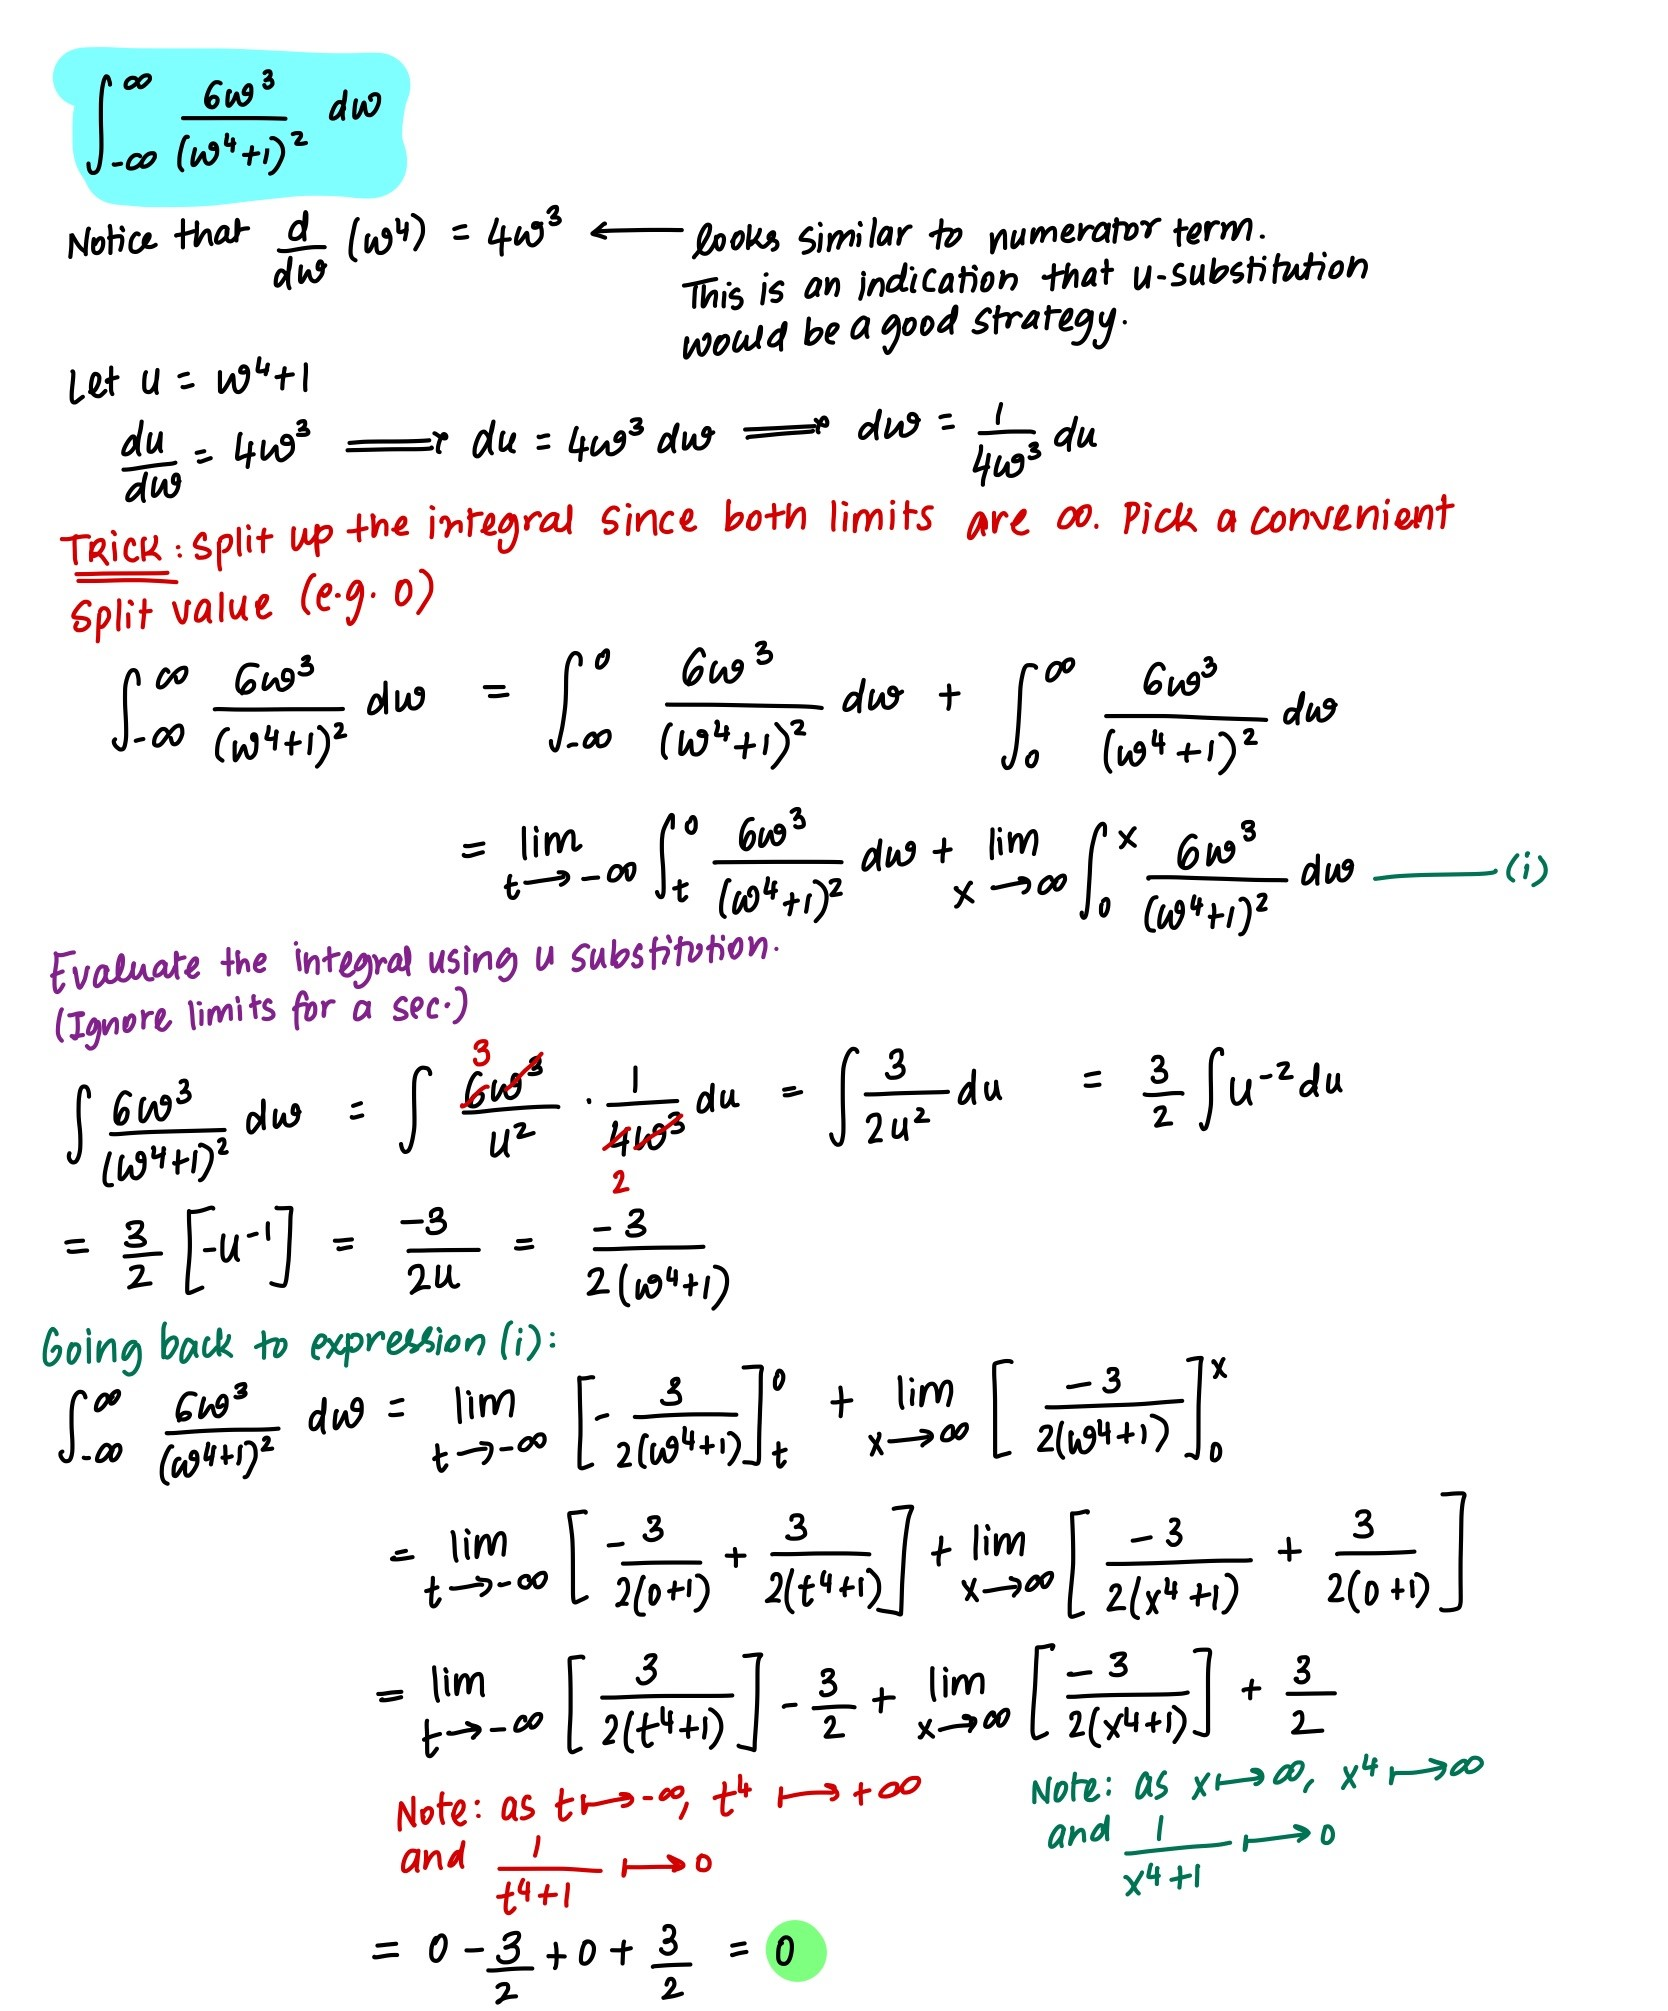
\includegraphics[width=0.95\linewidth]{Q3.jpg}
        \label{fig:Q3}
    \end{figure}
    \item $$\int_{-2}^2{\frac{1}{x^2}}dx$$
    \begin{figure}[H]
        \centering
        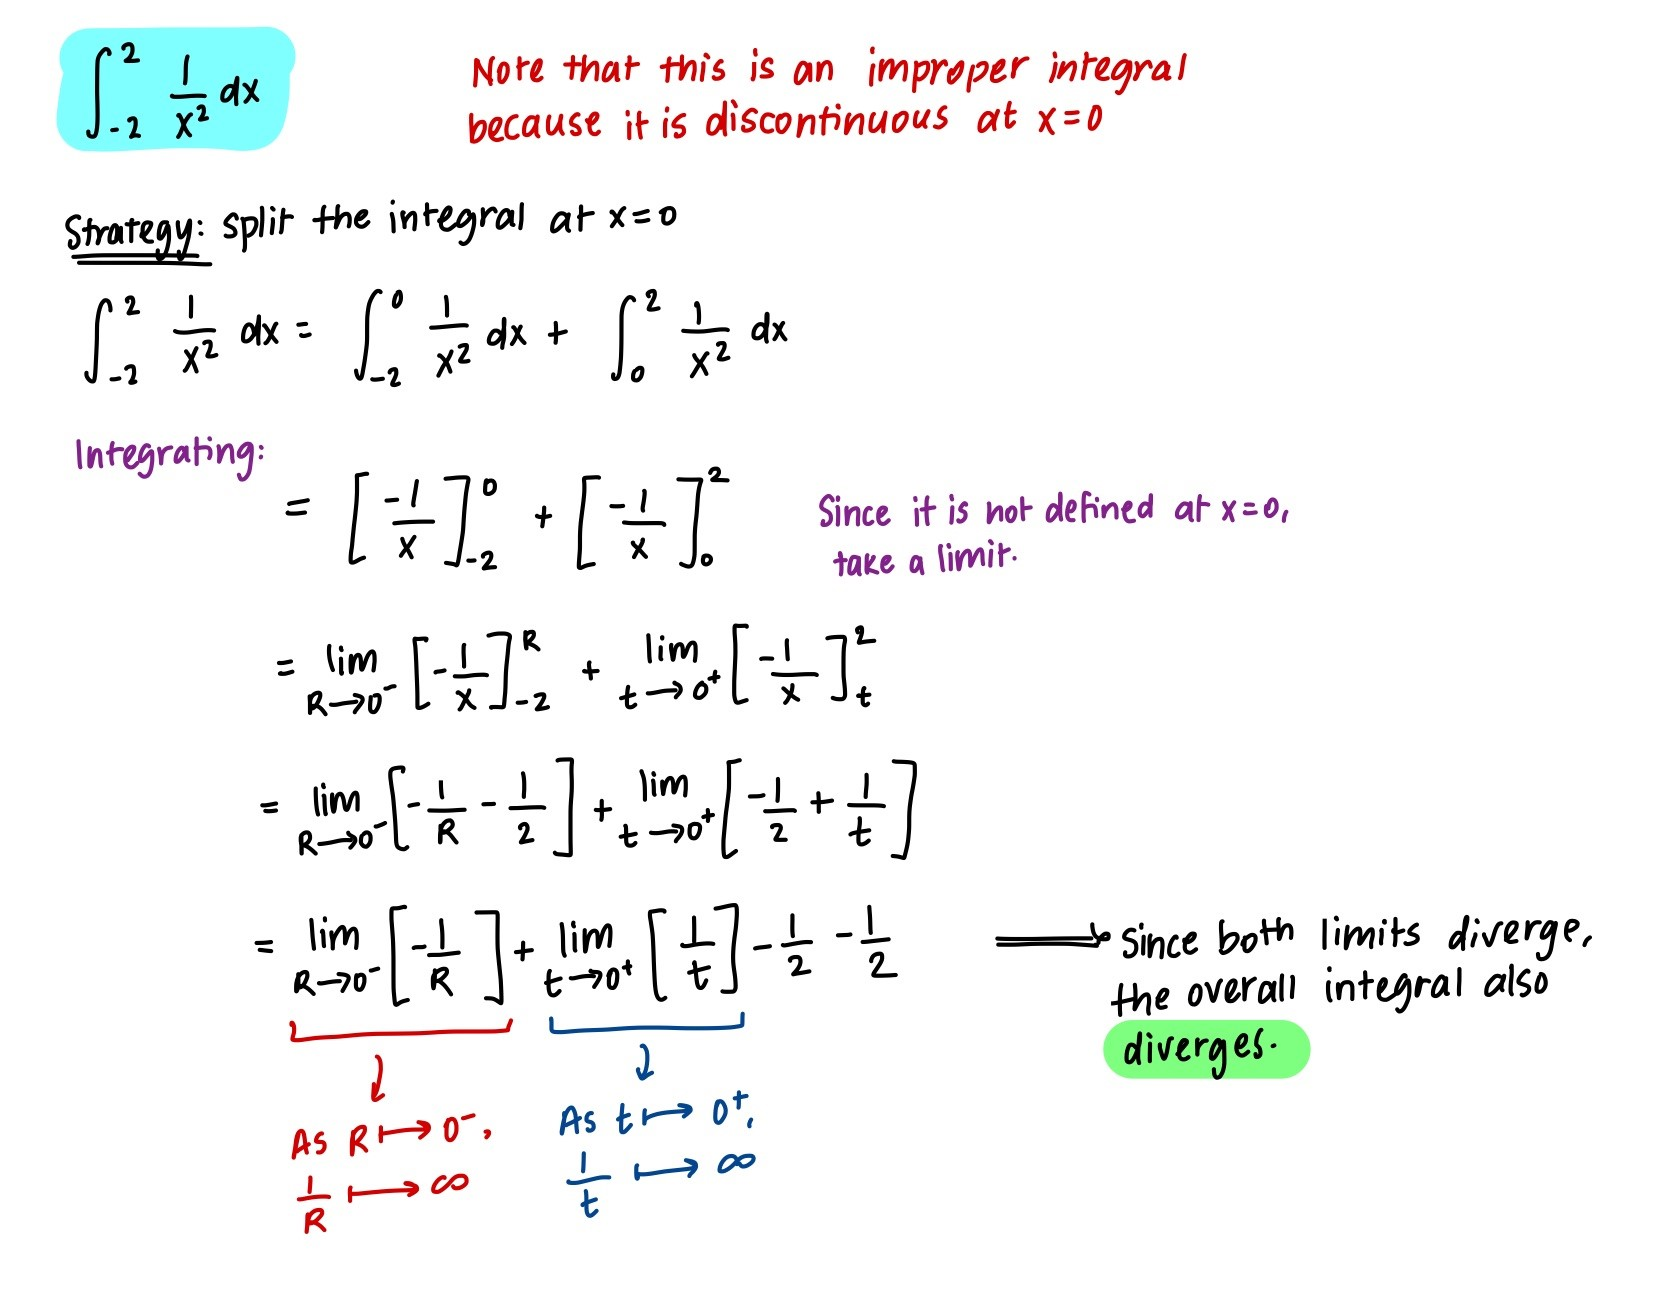
\includegraphics[width=\linewidth]{Q4.jpg}
        \label{fig:Q4}
    \end{figure}
    \newpage
    \item $$\int_{-\infty}^\infty{\cos(\pi t)}dt$$
    \begin{figure}[H]
        \centering
        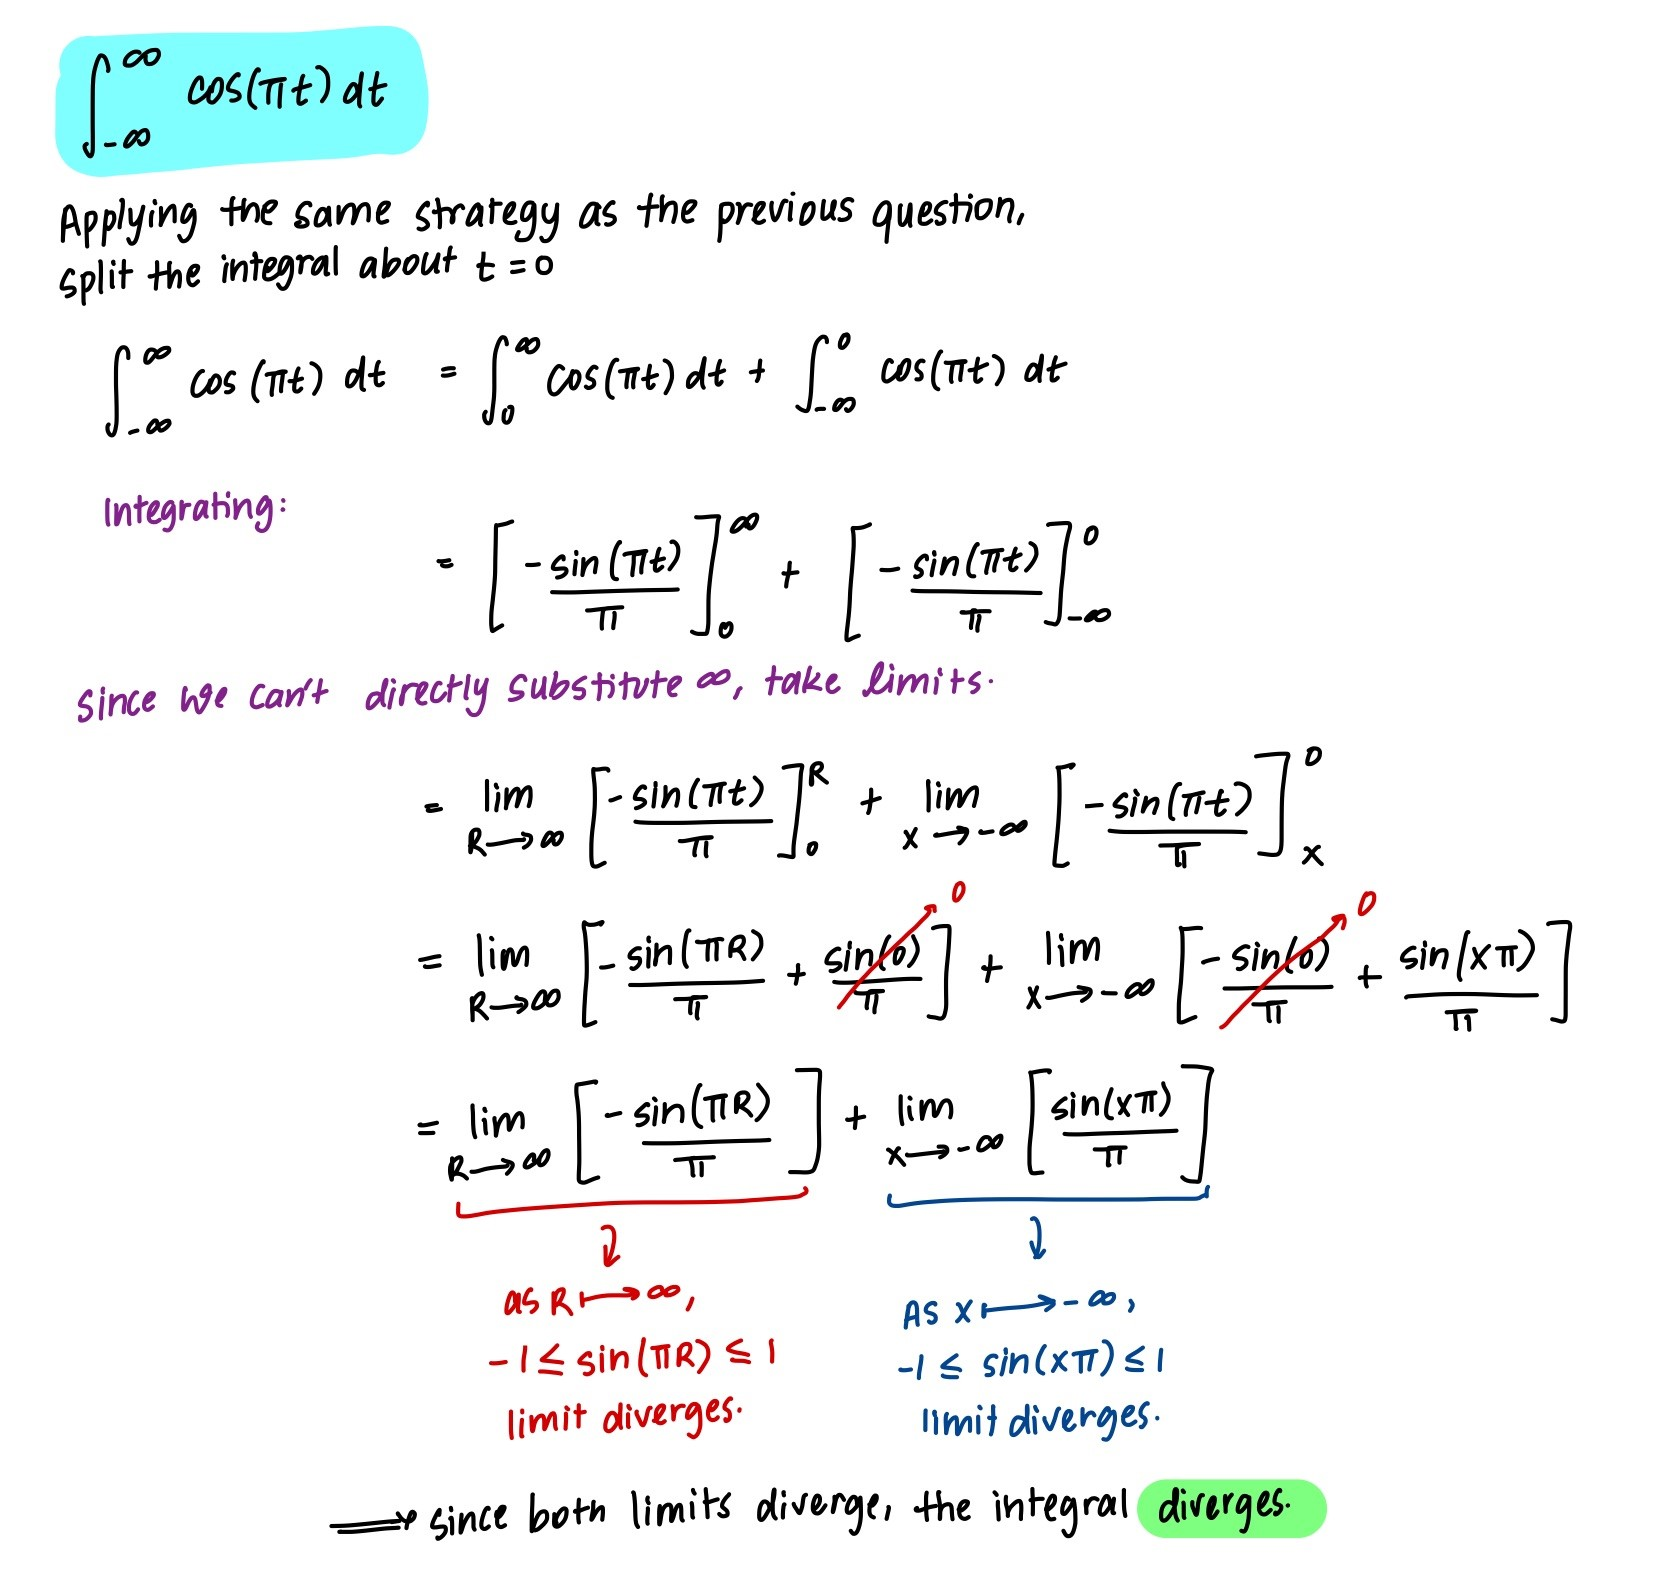
\includegraphics[width=\linewidth]{Q5.jpg}
        \label{fig:Q5}
    \end{figure}
    \newpage
    \item $$\int_0^\infty{\frac{e^x}{e^{2x}+3}}dx$$
    \begin{figure}[H]
        \centering
        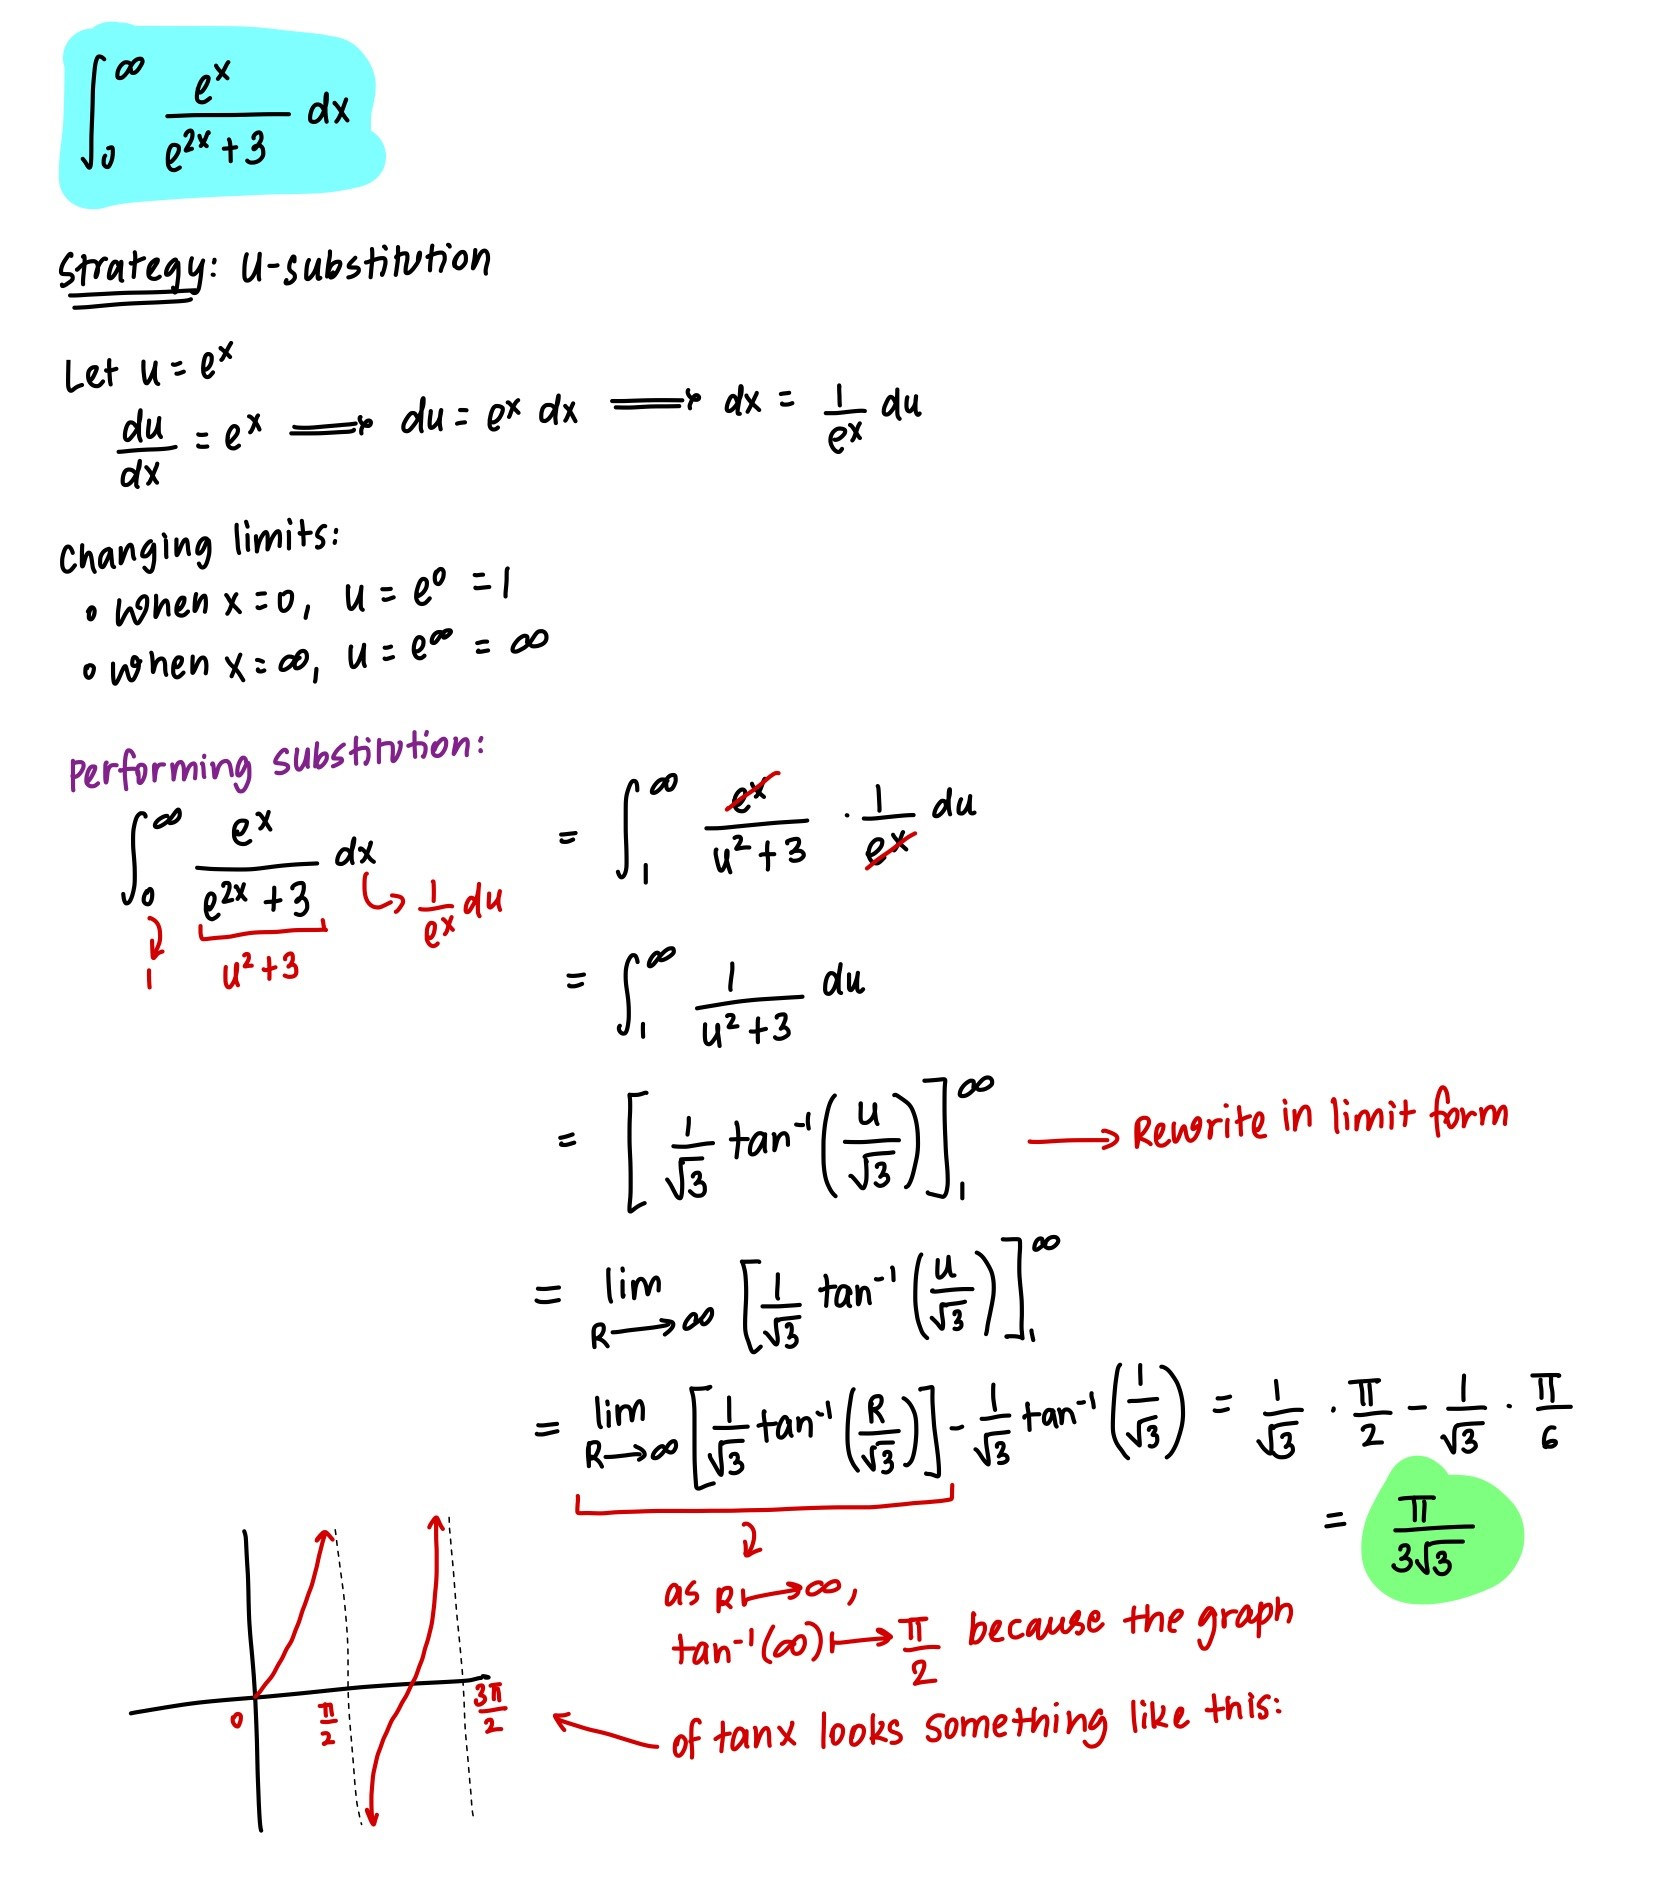
\includegraphics[width=\linewidth]{Q6.jpg}
        \label{fig:Q6}
    \end{figure}
    \item $$\int_1^\infty{\frac{\ln(x)}{x^2}}dx$$
    \begin{figure}[H]
        \centering
        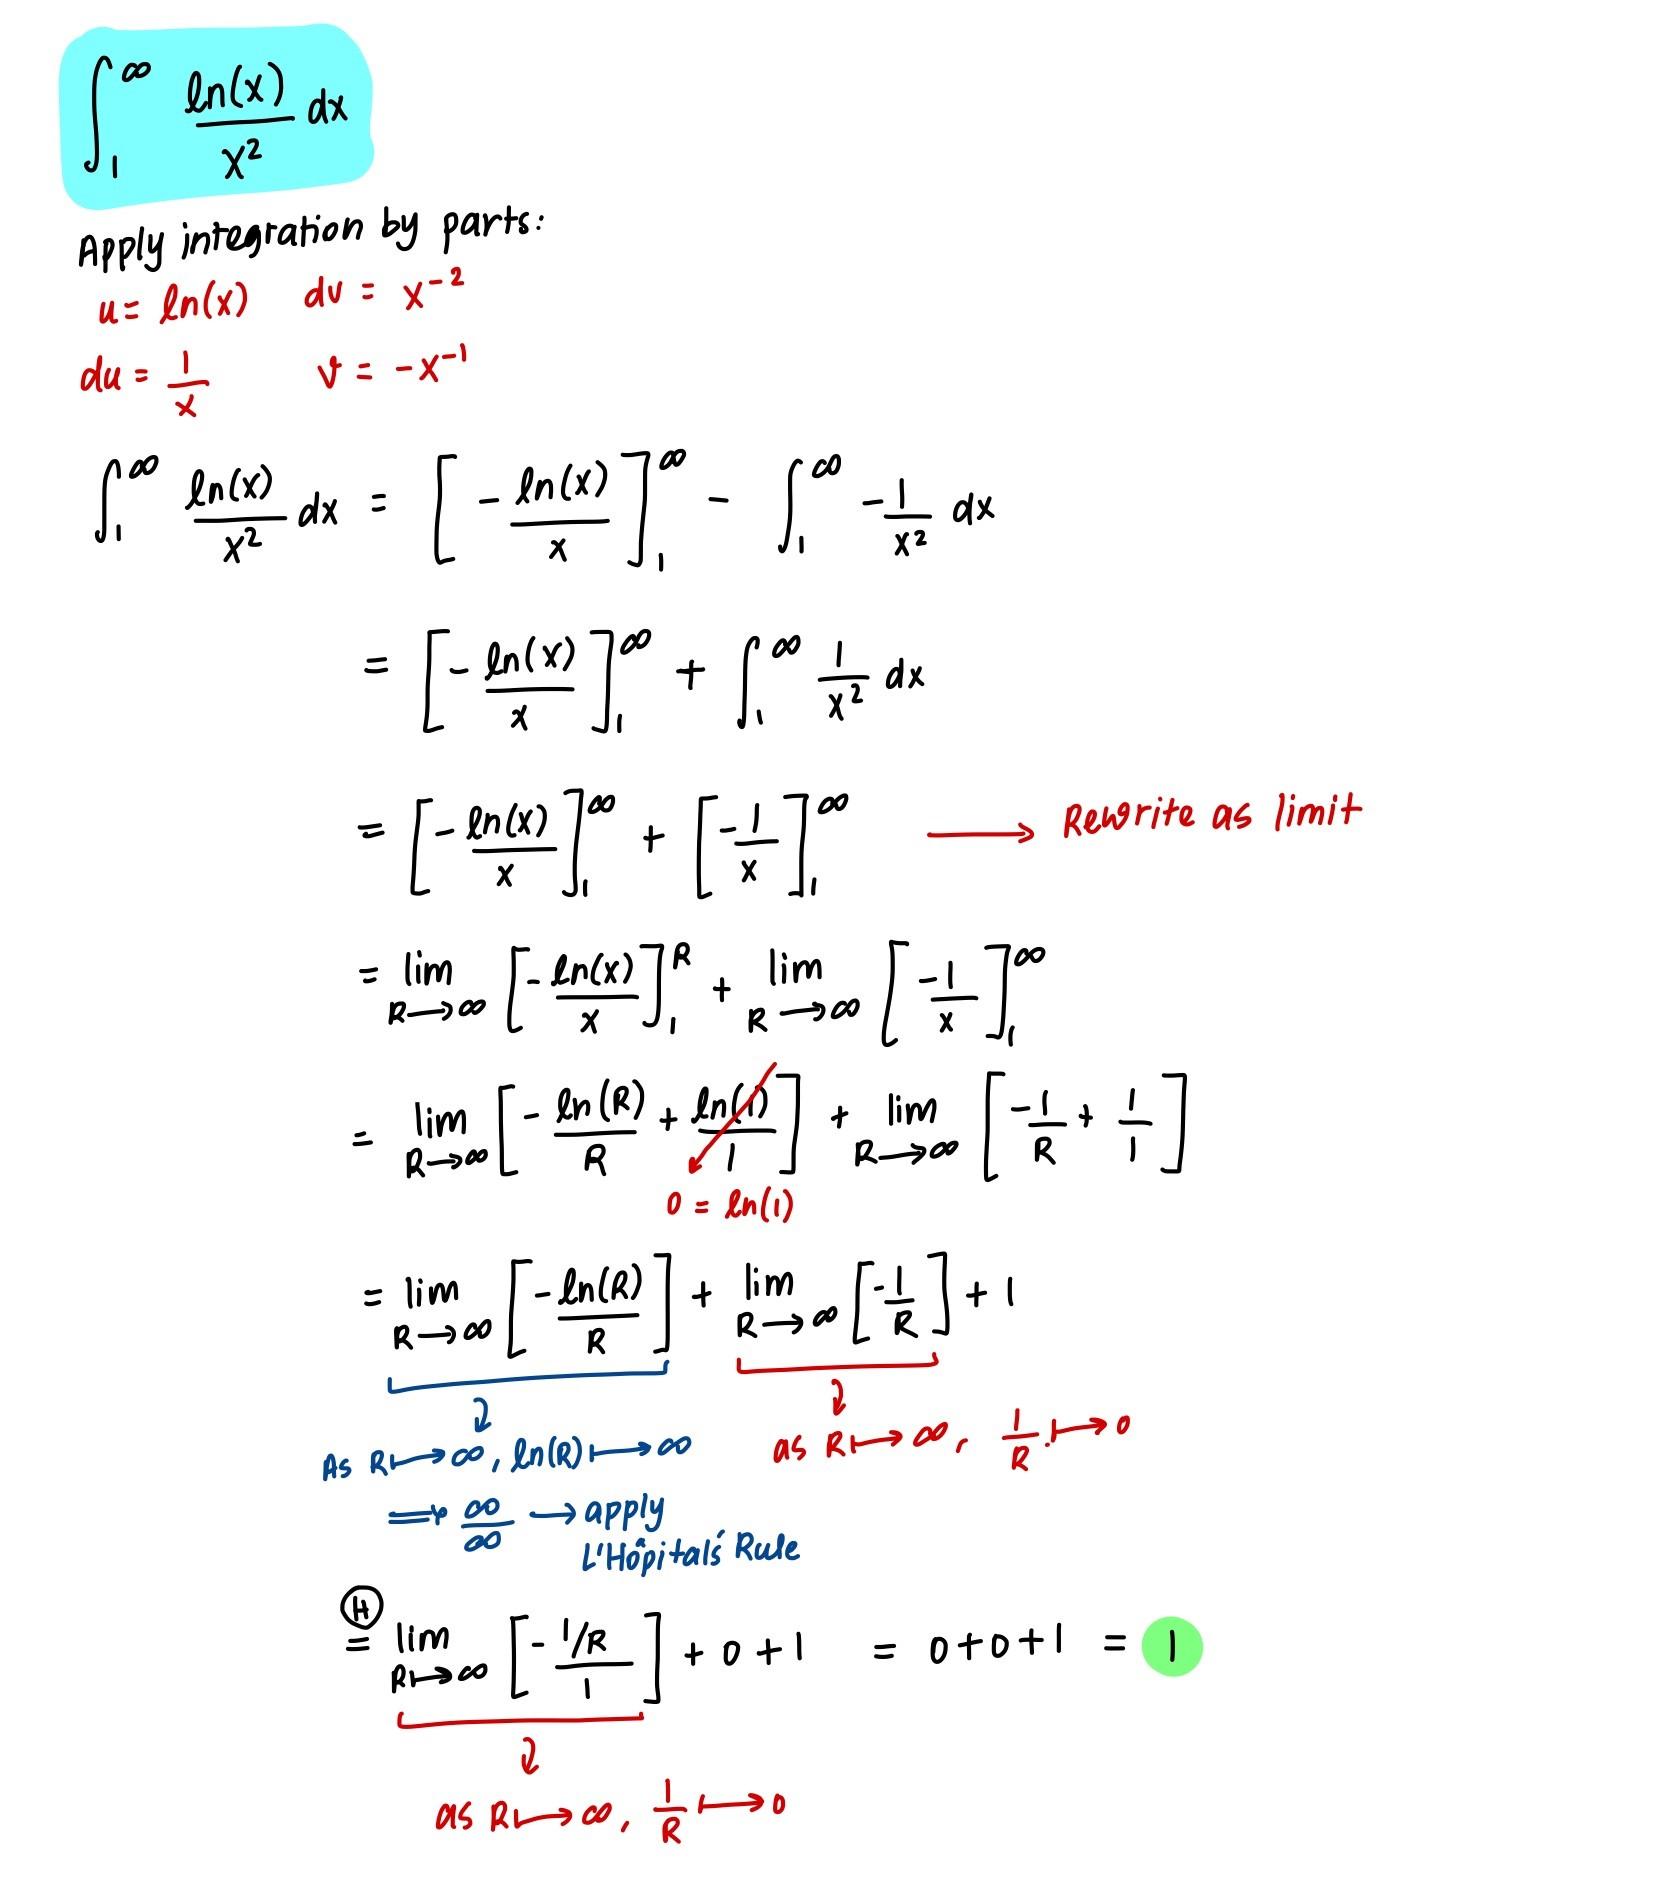
\includegraphics[width=\linewidth]{Q7.jpg}
        \label{fig:Q7}
    \end{figure}
    \item $$\int_0^\infty{\frac{1}{z^2+3z+2}}dz$$
    \begin{figure}[H]
        \centering
        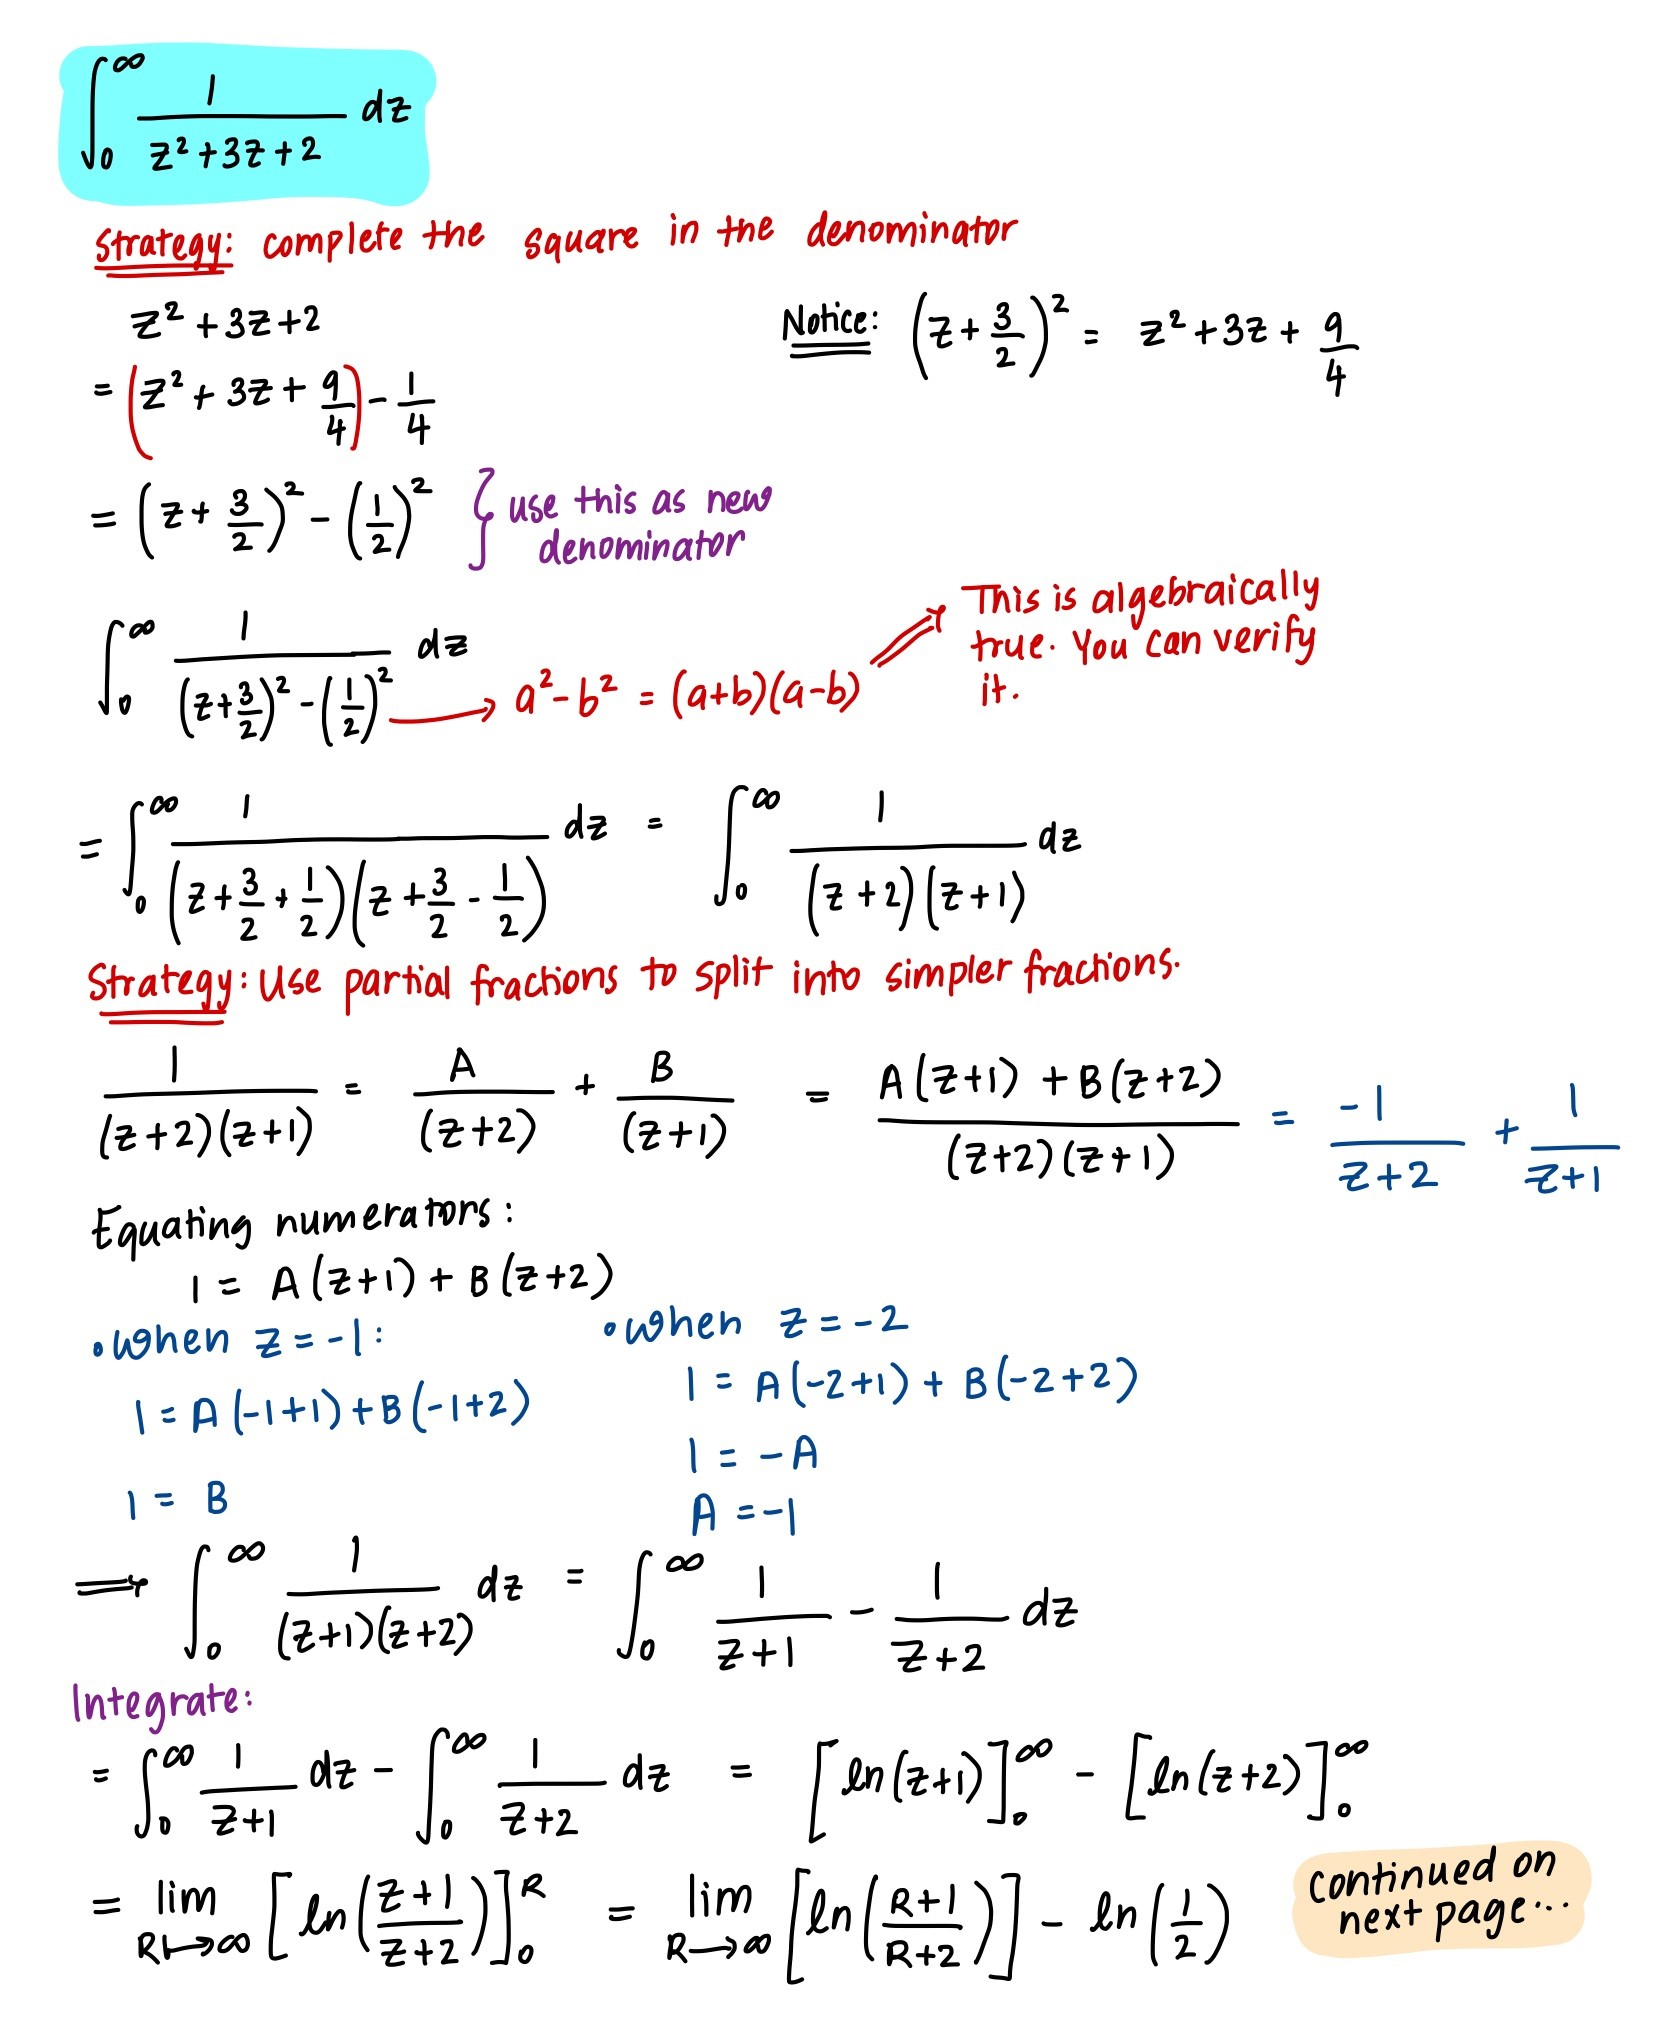
\includegraphics[width=0.95\linewidth]{Q8.1.jpg}
        \label{fig:Q8.1}
    \end{figure}
    \begin{figure}[H]
        \centering
        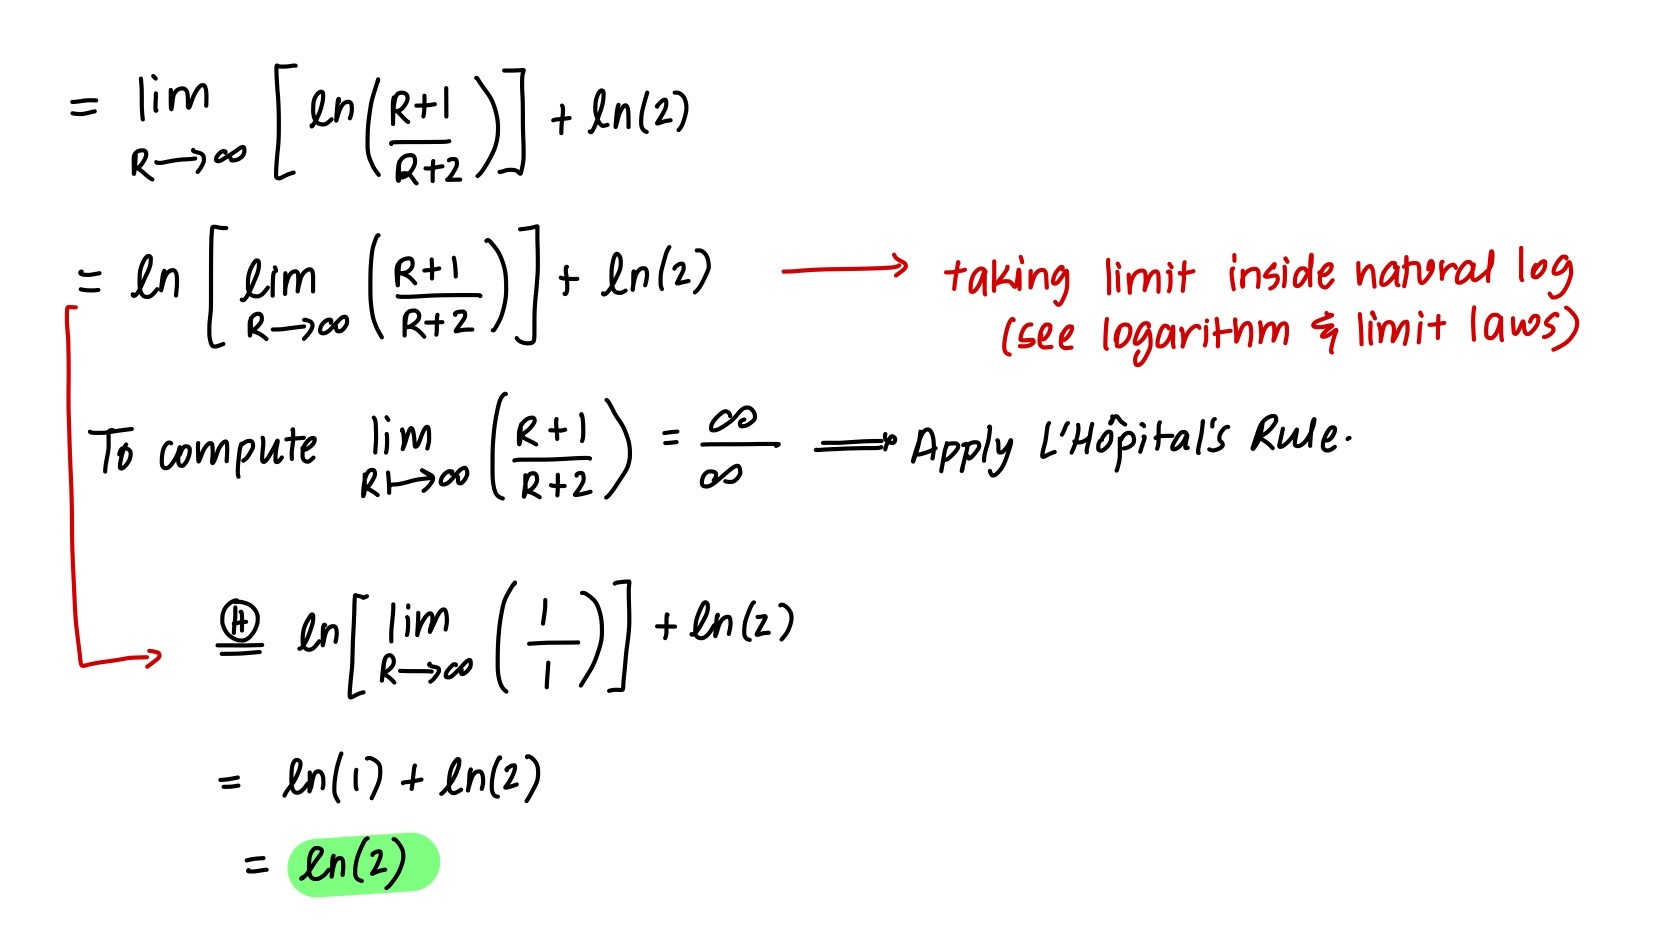
\includegraphics[width=\linewidth]{Q8.2.jpg}
        \label{fig:Q8.2}
    \end{figure}
\end{enumerate}

\end{document}
